\documentclass[crop,tikz]{standalone}

\usepackage{fontspec}
\setmainfont{texgyrepagella}[
  Extension = .otf,
  UprightFont = *-regular,
  BoldFont = *-bold,
  ItalicFont = *-italic,
  BoldItalicFont = *-bolditalic,
]

\usepackage{tikz}
\usetikzlibrary{decorations.pathreplacing,calligraphy}
\usetikzlibrary{calc}

\makeatletter % https://tex.stackexchange.com/a/38995/121799
\tikzset{
  use path/.code={\pgfsyssoftpath@setcurrentpath{#1}}
}
\makeatother
\tikzset{reverseclip/.style={insert path={(current bounding box.north
        east) rectangle (current bounding box.south west)}}}

\pgfdeclarelayer{bg}
\pgfsetlayers{bg,main}


\begin{document}
    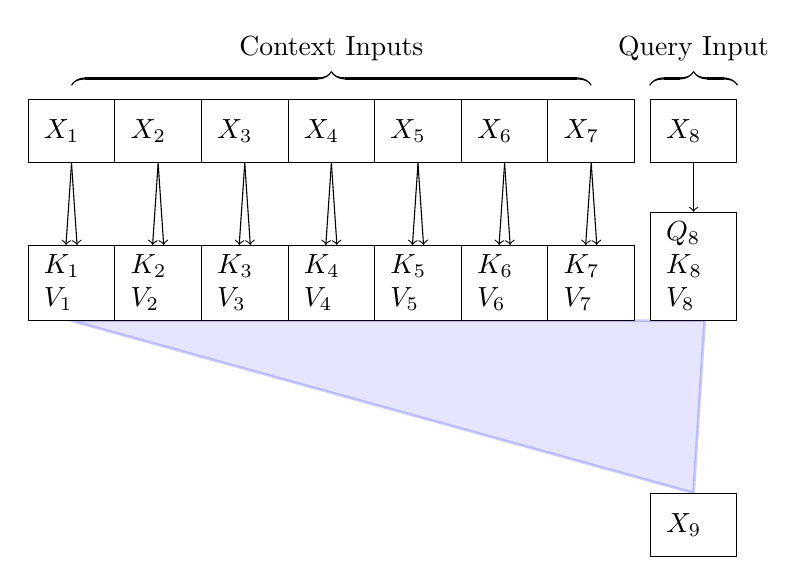
\begin{tikzpicture}
        \begin{scope}
            \tikzstyle{every node}=[draw,rectangle,text width=0.7cm, minimum width=1.1cm, minimum height=0.8cm]

            \begin{scope}[shift={(1.1cm * -3, 0)}]
                \begin{scope}[shift={(-3.4cm, 0)}]
                    \foreach \x in {1,...,7} {
                        \node[anchor=south] (x_\x) at (\x*1.1 cm, 0) {$X_{\x}$};
                    }
                \end{scope}
                \begin{scope}[shift={(-3.4cm, -2cm)}]
                    \foreach \x in {1,...,7} {
                        \node[transform shape,fill=white,anchor=south] (kv_\x) at (\x*1.1 cm, 0) {$K_{\x}$ $V_{\x}$};
                        \draw[->] (x_\x.south) -- ([xshift=-2pt]kv_\x.north);
                        \draw[->] (x_\x.south) -- ([xshift=2pt]kv_\x.north);
                    }
                \end{scope}
                \begin{scope}[shift={(4.5cm, 0)}]
                    \foreach \y / \i in {8/1} {
                        \node[anchor=south] (y_\y) at (\i*1.1 cm, 0) {$X_{\y}$};
                    }
                \end{scope}
                \begin{scope}[shift={(4.5cm, -2cm)}]
                    \foreach \y / \i in {8/1} {
                        \node[transform shape,fill=white,anchor=south] (q_\y) at (\i*1.1 cm, 0) {$Q_{\y}$ $K_{\y}$ $V_{\y}$};
                        \draw[->] (y_\y.south) -- (q_\y.north);
                    }
                \end{scope}
                \begin{scope}[shift={(4.5cm, -5cm)}]
                    \foreach \y / \yy / \i in {8/9/1} {
                        \node[transform shape,fill=white,anchor=south] (o_\y) at (\i*1.1 cm, 0) {$X_{\yy}$};

                        \begin{pgfonlayer}{bg}
                            \begin{scope}[
                            every path/.append style={draw=blue,fill=blue,fill opacity=0.1,draw opacity=0.2},
                            blend group=darken]
                                \fill[blue] (o_\y.north) -- (kv_1.south) -- ([xshift=4pt]q_\y.south) -- cycle;
                            \end{scope}
                        \end{pgfonlayer}
                    }
                \end{scope}
            \end{scope}
        \end{scope}
        \draw[thick,decorate,decoration={calligraphic brace,raise=5pt, amplitude=5pt}] (x_1.north) -- node[above=10pt] {Context Inputs} (x_7.north);
        \draw[thick,decorate,decoration={calligraphic brace,raise=5pt, amplitude=5pt}] (y_8.north west) -- node[above=10pt] {Query Input} (y_8.north east);

    \end{tikzpicture}
\end{document}
